
%(BEGIN_QUESTION)
% Copyright 2010, Tony R. Kuphaldt, released under the Creative Commons Attribution License (v 1.0)
% This means you may do almost anything with this work of mine, so long as you give me proper credit

A Koyo ``CLICK'' PLC monitors three process conditions (pressure, liquid level, and temperature) to turn on a solenoid valve when the right conditions are met:

$$\includegraphics[width=15.5cm]{i02269x01.eps}$$

Determine why the solenoid coil refuses to energize, based on the ``live'' display of the ladder logic program shown here:

$$\includegraphics[width=15.5cm]{i02269x02.eps}$$

Also, determine whether the I/O channels on this PLC are {\it sourcing} or {\it sinking} current.

\vskip 20pt \vbox{\hrule \hbox{\strut \vrule{} {\bf Suggestions for Socratic discussion} \vrule} \hrule}

\begin{itemize}
\item{} Supposed we wished to override the PLC and energize the solenoid coil.  How could this be done? Hint: there is more than one way to do this!
\end{itemize}

\underbar{file i02269}
%(END_QUESTION)





%(BEGIN_ANSWER)


%(END_ANSWER)





%(BEGIN_NOTES)

The solenoid is not energizing because the liquid level is too high, or else there is some other fault causing input {\tt X2} to be de-energized.  

\vskip 10pt

All inputs on this PLC are {\it sourcing}, while the output is {\it sinking}.

%INDEX% PLC, relating I/O status to virtual elements 

%(END_NOTES)


